\documentclass{beamer}
\usepackage[utf8]{inputenc}
\graphicspath{{./fig/}}

\title{Desenvolvimento Web Básico}
\subtitle{Aula 1}
\date{}

\usetheme{lucid}

\begin{document}
\frame{
 \titlepage
}

\frame{
    \frametitle{Roteiro de Aula}
    \tableofcontents
}

%-----------------------------------------------------------------------------------------
\section{A disciplina}
\begin{frame}{Começando...}
  \begin{itemize}
   \item Prof. Juliana Costa Silva
    \item E-mail: juliana.silva@up.edu.br
    \item Quem é a professora?
    \pause \item \textcolor{red}{Como a professora trabalha??}
  \end{itemize}
\end{frame}
%--------------------------------------------------------------------------------------
\begin{frame}{Começando [2]}
  \begin{itemize}
   \item Plano de aulas (Disponível para leitura);
   \item Chamada no final da aula;
    \item Trabalhos (projeto da disciplina, parte 1 e parte 2) - 2.0 pontos;
    \item Avaliação (prática + teórica) - 3.0 pontos: datas no plano de aulas;
  \end{itemize}
\end{frame}
%---------------------------------------------------------------------------------------
\begin{frame}{Sobre a WEB}
  \begin{enumerate}
   \item Você imagina como seria a vida sem internet?
    \item Como tantas informações ficam disponíveis na internet?
    \item Descreva como você vê o funcionamento de uma página WEB.
  \end{enumerate}
\end{frame}
%------------------------------------------------------------------------------------------
\begin{frame}
\frametitle{Roteiro} % Table of contents slide, comment this block out to remove it
\tableofcontents % Throughout your presentation, if you choose to use \section{} and \subsection{} commands, 
%these will automatically be printed on this slide as an overview of your presentation
\end{frame}
%-----------------------------------------------------------------------------
\section{Introdução}
\begin{frame}{Exibindo páginas WEB}
		\begin{center}
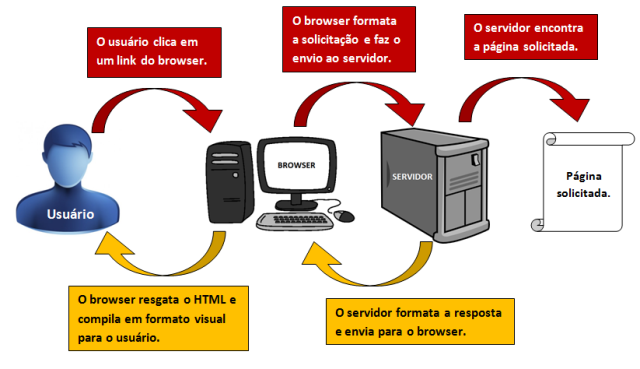
\includegraphics[height=0.65\paperheight]{fig/aula1/funcionamentoweb.jpg} \\
    		\tiny \textbf{Fonte:} \cite{freeman2008use}.
		\end{center}
\end{frame}
%-----------------------------------------------------------------------------
\begin{frame}{Exibindo páginas WEB}
  Como o navegador sabe o que exibir?
  \begin{block}{HTML}
    \begin{itemize}
      \item HTML - Hipertext Markup Language (Linguagem de Marcação de 
Hipertexto);
       \item Isto significa que é um código utilizado para descrever a 
estrutura de um documento, mas não é a verdadeira apresentação dele.
       \item O HTML diz ao navegador, tudo sobre o conteúdo recebido, e 
a estrutura da página;
       \item O HTML define cabeçalhos, parágrafos, listas, tabelas entre 
muitos outros elementos, por meio de marcas (\textit{tags}).
    \end{itemize}
    \tiny{Fonte: \cite{marinho2016}}
  \end{block}
\end{frame}
%-----------------------------------------------------------------------------
\section{HTML}
\begin{frame}{Tags HTML}
  \begin{center}
    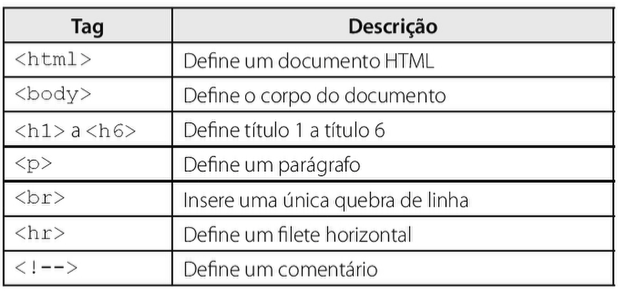
\includegraphics[height=0.5\paperheight]{fig/aula1/tagBasica.png}\\
    \tiny{Fonte: \cite{marinho2016}.}
   \end{center}
\end{frame}
%-----------------------------------------------------------------------------
\begin{frame}{O que é uma TAG?}
  \begin{center}
    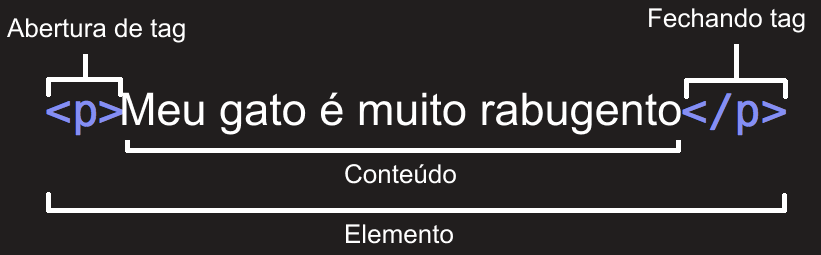
\includegraphics[height=0.28\paperheight]{fig/aula2/aula2_tag.png}\\
    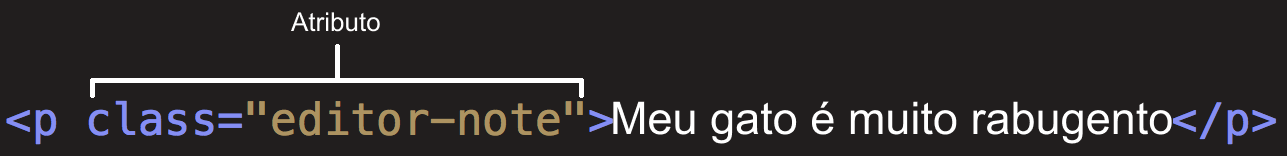
\includegraphics[height=0.13\paperheight]{fig/aula2/aula2_tag2.png}\\
    \tiny{Fonte: \cite{mdn2023}.}
   \end{center}
\end{frame}
%-----------------------------------------------------------------------------
\begin{frame}{HTML}
  O navegador lê o código HTML e, interpreta todas as \textit{tags}. \\
   \textbf{tags:} Palavras entre os sinais de maior e menor, como: 
$<head>$ ou $<p>$.
\end{frame}
%----------------------------------------------------------------
\begin{frame}{Estrutura}
  \begin{block}{Estrutura de uma página HTML}
    Toda página html, por mais simples que seja, deve conter as seguintes tags 
elementares:
    \begin{itemize}
     \item $<html>$: é a tag que identifica o documento como um hipertexto html;
     \item $<head>$: é a tag que apresenta informações gerais sobre a 
página e de configuração;
     \item $<title>$: é a tag que informa o título de uma página na barra 
do navegador;
     \item $<body>$: é a tag que delimita o conteúdo da página;
  \end{itemize}
  \end{block}
\end{frame}
%---------------------------------------------------------
\begin{frame}{Estrutura II}
  \begin{block}{Estrutura de uma página HTML}
   \begin{itemize}
    \item Além disso, a tag a seguir define a codificação de caracteres 
para o padrão UTF-8: $<$meta charset = “UTF-8” $/>$ \\
   \item A instrução a seguir indica para o navegador utilizar a versão 
mais recente do HTML (HTML5):
  \item $<$!DOCTYPE html$>$
  \end{itemize}
  \end{block}
\end{frame}
%---------------------------------------------------
\frame {
 \frametitle{Linguagens básicas WEB}
 \framesubtitle{Breve apresentação}
 \begin{itemize}
     \item \textbf{HTML} é a linguagem de marcação que nós usamos para estruturar e dar significado para o nosso conteúdo web. Por exemplo, definindo parágrafos, cabeçalhos, tabelas de conteúdo, ou inserindo imagens e vídeos na página.\\
     \textbf{CSS} é uma linguagem de regras de estilo que nós usamos para aplicar estilo ao nosso conteúdo HTML. Por exemplo, definindo cores de fundo e fontes, e posicionando nosso conteúdo em múltiplas colunas.\\
     \textbf{JavaScript} é uma linguagem de programação que permite a você criar conteúdo que se atualiza dinamicamente, controlar multimídias, imagens animadas. 
 \end{itemize}
}

%---------------------------------------------------------------------------------
\begin{frame}{Tag: Títulos}
  \begin{columns}
    \begin{column}{0.5\textwidth}
      Para indicar que um texto é um título em nossa página,
utilizamos a tag de heading;\\

      São tags de conteúdo e vão de $<$h1$>$ até $<$h6$>$;\\
 
    A variação entre as tags de heading definem o grau de destaque do texto;
   \end{column}
   \begin{column}{0.4\textwidth}
    \begin{center}
      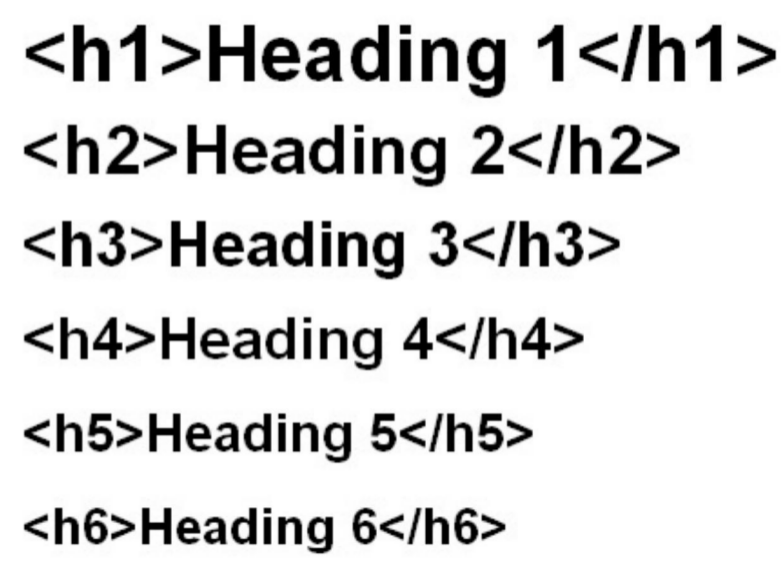
\includegraphics[height=0.4\paperheight]{fig/aula1/heading.png} \\
    \end{center}
   \end{column}
  \end{columns}
  
  Acrescente Três títulos a sua página!
\end{frame}
%-------------------------------------------------------------------------
\begin{frame}{Tags de formatação}
 As seguintes tags são utilizadas para a apresentação de conteúdo textual em 
uma 
página:
\begin{itemize}
 \item $<$p$>$: tag para a representação de um parágrafo;
  \item $<$span$>$: tag para representar um texto sem significado (deve 
ser usado quando nenhum outro elemento de texto semântico representar um 
significado adequado);
   \item Outros;
\end{itemize}
\end{frame}
%-------------------------------------------------------------------------
\begin{frame}{Tags de texto}
 Teste as Tags abaixo no seu arquivo html e descreva o que cada uma faz
\begin{itemize}
 \item $<$strike$>$
  \item $<$sub$>$
  \item $<$sup$>$
  \item $<$big$>$
  \item $<$small$>$
  \item $<$tt$>$
  \item $<$pre$>$
  \item $<$cite$>$
  \item $<$strong$>$
  \item $<$em$>$
  \item $<$blockquote$>$
  \item $<$q$>$
\end{itemize}
\end{frame}
%-----------------------------------------------------------
\begin{frame}{Detalhando...}
 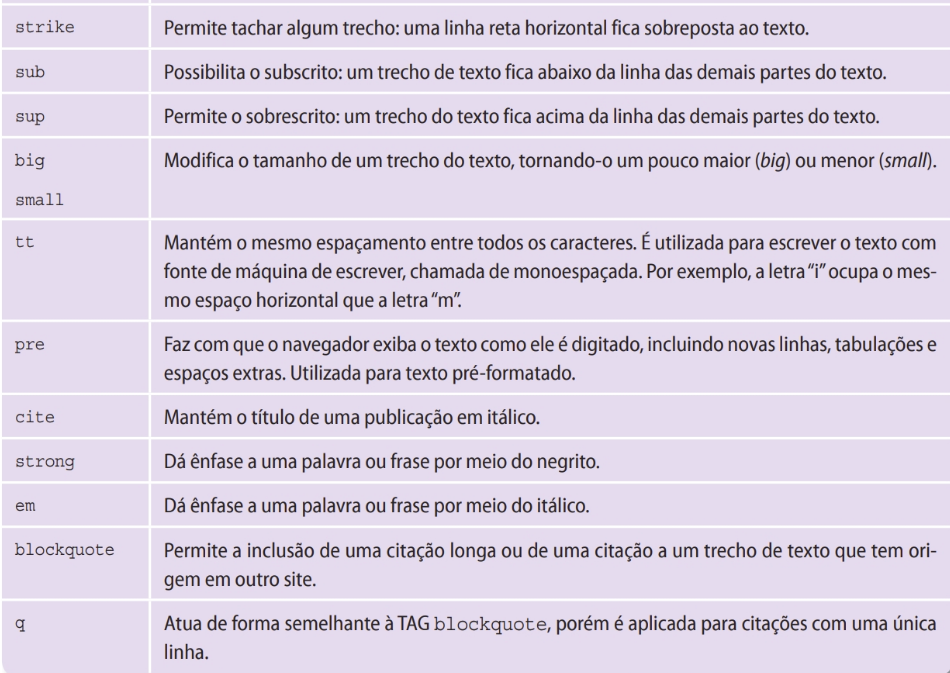
\includegraphics[height=0.7\paperheight]{fig/aula1/tagFormata.png} \\
\end{frame}

%-----------------------------------------------------------------------------
\section{Listas}
\begin{frame}{Tags HTML - Listas}
  Listas são utilizada em diversas ocasiões em uma página HTML;
  \begin{itemize}
   \item A apresentação de itens do um assunto (como esse slide);
   \item Estruturação de novos componentes (como um menu);
  \end{itemize}
   Existem três tipos de listas no HTML:
  \begin{enumerate}
   \item Listas ordenadas;
    \item Listas não ordenadas;
    \item Listas de definições;
 \end{enumerate}
 Também é possível criar listas aninhadas.\\
 \tiny{Fonte: \cite{miletto2014desenvolvimento}}
\end{frame}
%---------------------------------------------------------------------------------
\subsection{Lista ordenada}
\begin{frame}{Lista ordenada}
  \begin{columns}
    \begin{column}{0.45 \textwidth}
     \begin{itemize}
      \item Cria uma lista que segue uma sequência numérica;
       \item Utiliza a tag $<$ol$>$ (\textit{ordered list});
       \item Cada item da lista é expresso entre a tag $<$li$>$ 
      (\textit{list item});
     \end{itemize}
    \end{column}
    \begin{column}{0.5\textwidth}
     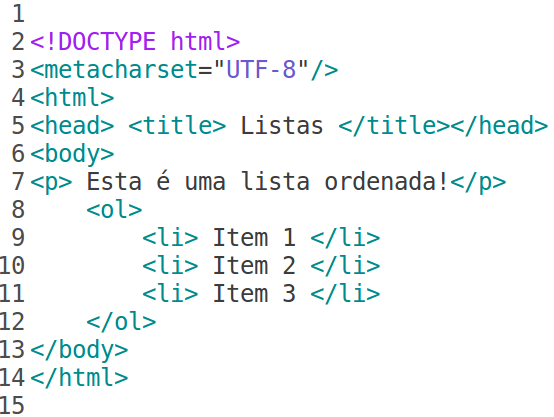
\includegraphics[height=0.45\paperheight]{fig/aula1/html2.png}
    \end{column}
  \end{columns}
\end{frame}
%---------------------------------------------------
\subsection{Lista desordenada}
\begin{frame}{Lista desordenada}
  \begin{columns}
    \begin{column}{0.45 \textwidth}
     \begin{itemize}
      \item Cria uma lista que não segue uma sequência.
       \item Utiliza a tag $<$ul$>$ (\textit{unordered list});
       \item Cada item da lista é expresso entre a tag $<$li$>$ 
      (\textit{list item});
     \end{itemize}
    \end{column}
    \begin{column}{0.5\textwidth}
     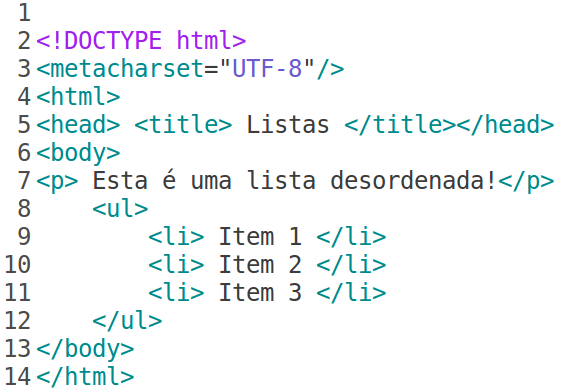
\includegraphics[height=0.45\paperheight]{fig/aula1/html3.png}
    \end{column}
  \end{columns}
\end{frame}

%---------------------------------------------------------------------
\section{Referências}
\begin{frame}{Referências}%[allowframebreaks]
\frametitle{Referências}
\small
\begin{center}
\tiny
\bibliographystyle{apalike}
\bibliography{./ref_aula}
\end{center}
\end{frame}


\end{document}